\begin{vbframe}{Linear Models -- Functionality}

\maketag{SUPERVISED} \maketag{PARAMETRIC} \maketag{WHITE-BOX}
\medskip

\highlight{General idea} ~~ Represent target as function of linear predictor
$\thx$

\medskip

\highlight{Hypothesis space}

$\Hspace = \left\{f: \Xspace \to \R ~|~\fx = \phi(\thetab^\top \xv)\right\}$, 
with suitable transformation $\phi(\cdot)$, e.g.,

\begin{itemize}
  \item Identity $\phi(\thetab^\top \xv) = \thetab^\top \xv$ 
  ~ $\Rightarrow$ \textbf{linear regression}
  % $\rightarrow$ continous output
  \item Logistic sigmoid function $\phi(\thx) = \frac{1}{1 + \exp(- \thx)} 
  =: \pixt$
  ~ $\Rightarrow$ \textbf{(binary) logistic regression}
  \begin{itemize}
    \footnotesize
    \item Probability $\pixt = \post$ of belonging to one of two classes
    \item Separating hyperplane via decision rule 
    (e.g., $\yh = 1 \Leftrightarrow \pix > 0.5$)
  \end{itemize}
\end{itemize}

\begin{minipage}[b]{0.32\textwidth}
  \begin{center}
% from FCIM: lecture_cim2\2020\02-univariate-modelling\archive\slides-2-multi-linear.Rnw
    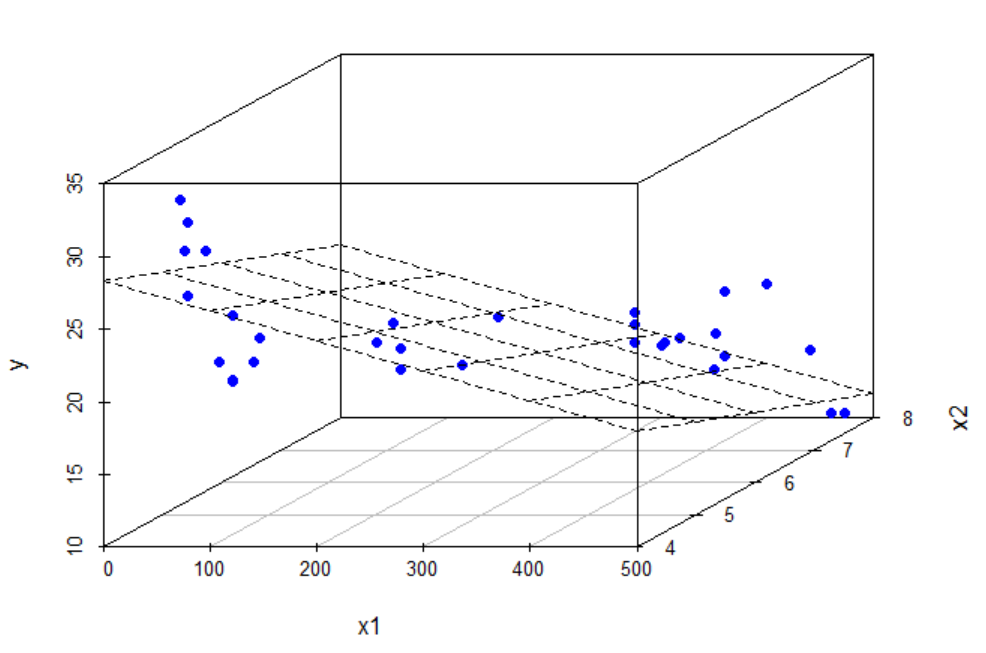
\includegraphics[height=0.6\textwidth,keepaspectratio=true]{
    figure/linreg-surface.png} \\
    \tiny{Linear regression hyperplane}
  \end{center}
\end{minipage}
\begin{minipage}[b]{0.32\textwidth}
  \begin{center}
% from FCIM: lecture_cim2\2020\02-univariate-modelling\figure_man
    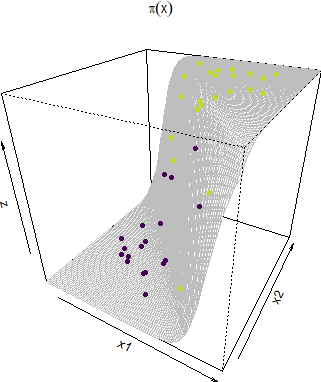
\includegraphics[height=0.6\textwidth, keepaspectratio=true]{
    figure/logreg-2vars-surface.png}\\
    \tiny{Logistic function for bivariate input}
  \end{center}
\end{minipage}
\begin{minipage}[b]{0.32\textwidth}
  \begin{center}
  % from FCIM: lecture_cim2\2020\02-univariate-modelling\figure_man
    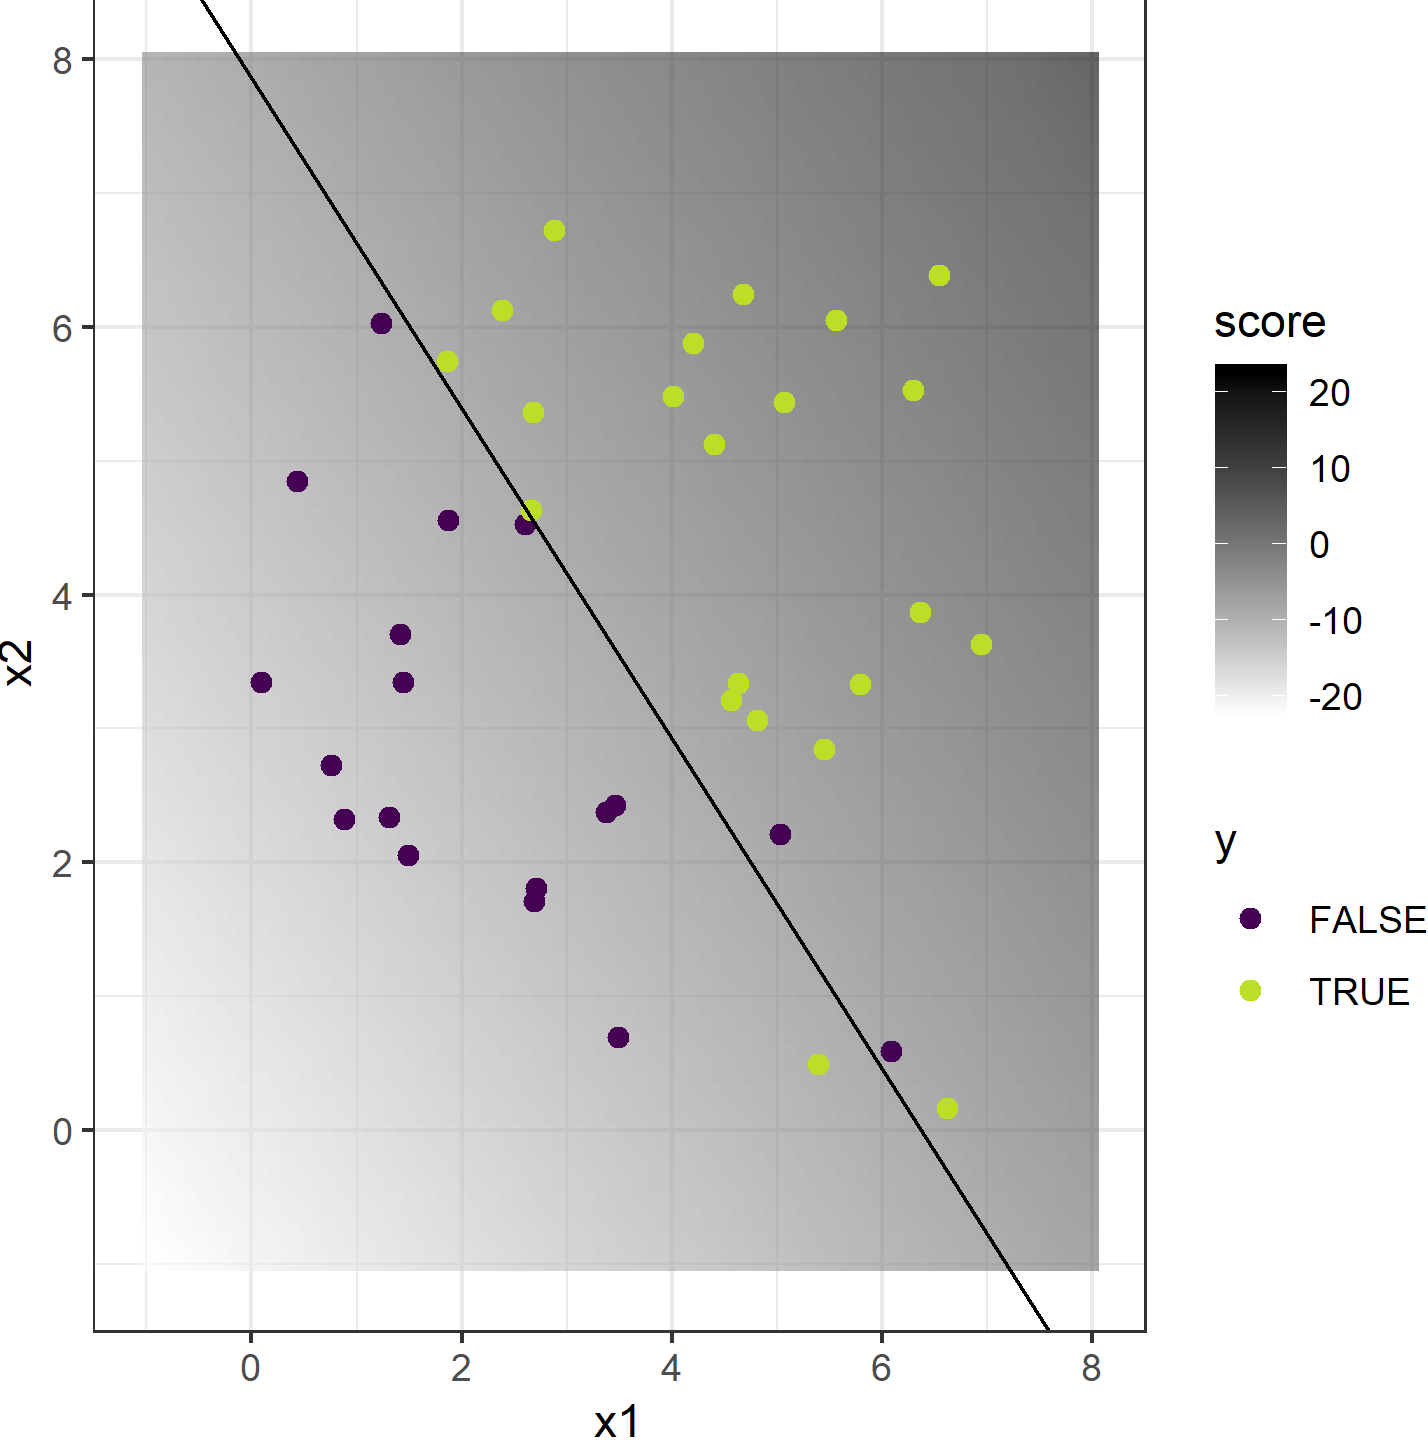
\includegraphics[height=0.6\textwidth, keepaspectratio=true]{
    figure/logreg-2vars-data.png} \\
    \tiny{Separating hyperplane for bivariate logistic regression}
\end{center}
\end{minipage}

\framebreak

\highlight{Empirical risk}

\begin{itemize}
  \item \textbf{Linear regression}
  \begin{itemize}
    \footnotesize
    \item Typically, based on \textbf{quadratic} loss: $\risket = 
    \sumin \left(\yi - \fxit \right)^2$ \\
    $\Rightarrow$ corresponding to ordinary-least-squares (OLS) estimation
    \item Alternatives: e.g., \textbf{absolute} or \textbf{Huber} loss (both 
    improving robustness)
  \end{itemize}
  \item \textbf{Logistic regression:} based on 
  \textbf{Bernoulli/log/cross-entropy} loss ~ 
  $\Rightarrow \risket = \sumin -\yi \log 
  \left(\pixii\right) - (1 - \yi) \log \left(1 - \pixii \right)$
\end{itemize}

\medskip

\highlight{Optimization}
\begin{itemize}\footnotesize
  \item For \textbf{OLS}: analytically with 
  $\thetabh = \olsest$ \\
  (with $\Xmat \in \R^{n \times p}$ : matrix of feature vectors)
  \item For \textbf{other loss functions}: numerical optimization 
\end{itemize}

\medskip

\highlight{Hyperparameters} ~~ None

\medskip

% \highlight{Runtime behavior} ~~ $\mathcal{O}(p^2 \cdot n + p^3)$ for $n$ 
% observations and $p$ features

\end{vbframe}

% ------------------------------------------------------------------------------

\begin{frame}{Linear Models -- Pro's \& Con's}

\footnotesize

\begin{columns}[onlytextwidth]
  \begin{column}{0.5\textwidth}
    \highlight{Advantages}
    \footnotesize
    \begin{itemize}
      \positem \textbf{simple and fast} implementation
      \positem \textbf{analytical} solution
      \positem \textbf{cheap} computation
      \positem applicable for any \textbf{dataset size}, as long as number of 
      observations $\gg$ number of features
      \positem flexibility \textbf{beyond linearity} with polynomials, 
      trigonometric transformations etc.
      \positem intuitive \textbf{interpretability} via feature effects
      % \positem fits \textbf{linearly} separable data sets very well
      \positem statistical hypothesis \textbf{tests} for effects available

    \end{itemize}
  \end{column}

  \begin{column}{0.5\textwidth}
    \highlight{Disadvantages}
    \footnotesize
    \begin{itemize}
      \negitem \textbf{nonlinearity} of many real-world problems
      \negitem further restrictive \textbf{assumptions}: linearly independent 
      features, homoskedastic residuals, normality of conditional response
      \negitem \textbf{sensitivity} w.r.t. outliers and noisy data (especially 
      with L2 loss)
      \negitem risk of \textbf{overfitting} in higher dimensions
      \negitem feature \textbf{interactions} must be handcrafted, so higher
      orders practically infeasible
      \negitem no handling of \textbf{missing} data
    \end{itemize}
  \end{column}
\end{columns}

\vfill

\small

\conclbox{Simple method with good interpretability for linear problems, but with 
strong assumptions and limited complexity}

\end{frame}

% ------------------------------------------------------------------------------

\begin{frame}{Linear Models -- Practical hints}

\footnotesize

%% WOULD DELTETE THIS!
%  \highlight{\textcolor{blue}{Check assumptions??} }\\
% Linear models are effective if the following assumptions are fulfilled:
%  \begin{itemize}\footnotesize
%   \item \textbf{linearity}: The expected response is a linear combination of the features.
%   \item \textbf{homoscedasticity}: The variance of residuals is equal for all features.
%   \item \textbf{independence}: All observations are independent of each other.
%   \item \textbf{normality}: Y is normally distributed for any fixed value of the features
% \end{itemize}

\highlight{Implementation}

\begin{itemize}
  \item \textbf{R:} \texttt{mlr3} learner \texttt{LearnerRegrLM}, calling 
  \texttt{stats::lm()} / \texttt{mlr3} learner \texttt{LearnerClassifLogReg}, 
  calling \texttt{stats::glm()}
  \item \textbf{Python:} \texttt{LinearRegression} from package 
  \texttt{sklearn.linear\_model}, package for advanced statistical parameters 
  \texttt{statsmodels.api} 
\end{itemize}

\medskip

\highlight{Regularization}

\begin{itemize}
  \item Quadratic penalty on model coefficients (a.k.a. \textbf{Ridge} 
  regression)
  \begin{itemize} \footnotesize
    \item Overall smaller, but still dense $\thetab$
    \item Suitable with many influential features present, handling correlated 
    features by shrinking their coefficients equally
  \end{itemize}
  \item Absolute penalty on model coefficients (a.k.a. \textbf{Lasso} 
  regression)
  \begin{itemize} \footnotesize
    \item Actual variable selection
    \item Suitable for sparse problems, ineffective with correlated 
    features (randomly selecting one)
  \end{itemize}  
  \item Weighted combination of Ridge and Lasso: \textbf{elastic net}
\end{itemize}

\end{frame}